\chapter{Background and Related Works}
\label{Background and Related Works}
\section{Cassandra}

Cassandra is a widely used distributed \gls{nosql} database with many use cases \cite{Lakshman2010CassandraSystem}.  Not only has Cassandra been reportedly been used in practice \cite{ApacheCases}, but has been, using the Yahoo Cloud Services Benchmark \cite{YahooBenchmark}, formally evaluated in scholarly literature against other databases such as MongoDB and proposed as the NoSQL database of choice in the Internet of Things and distributed sensor networks \cite{Abramova2013NoSQLCassandra}.  There have been credible claims of Cassandra being used on Raspberry Pi \cite{VanRyswykMulti-DatacenterPis,SercelCassandraMedium}, but to the author's knowledge, no white paper with the details exists.  The aim of this paper is to examine Cassandra's performance coupled with a simplified Wi-Fi collection and analysis application, where the nature of link nodes may be less reliable than wired Ethernet.

This author's interest in Cassandra lies in the fact that Cassandra is a distributed database used in practice for cloud computing.  Although it describes itself as a NoSQL database, the interface allows for SQL commands and has a Python API.  Cassandra allows for configuration of distributed systems parameters, such as replication factor, but detailed knowledge of distributed systems protocols is not critical for operation.

From an experimental standpoint, the distributed nature of a Cassandra "keyspace" lies in four parameters \cite{CassandraDummies}: cluster size (the number of nodes), replication factor (configured in software), write level (configured in software), and read level (configured in software).

\section{Raspberry Pi 2}

The Raspberry Pi 2 (Model B) \cite{RaspberryB} is a low-cost computer designed sold from the United Kingdom.
It can be described as a motherboard for a about the size of a 3x5 index card and has been available since February 2015.
This experiment is interested in the Raspberry Pi 2 as a representative of the low-cost hardware domain, which implies low cost, low power consumption, and low in terms of size and weight.

This author's interest in the Raspberry Pi 2 is that its ARM Cortex-A7 processor and 1GB RAM \cite{RaspberryB} makes it a key representative of the low-cost hardware domain and \gls{iot}.
The Raspberry Pi 2 has cost as low as 35 USD \cite{RaspberryPi}. It is lightweight and has limited power consumption \cite{RaspberryB}. Constraints on size, weight, power, and cost can all be barriers to entry for applications seeking computing nodes.

Expanding this experiment, to say the BeagleBone black \cite{BeagleBoard.orgBlack}, is in touch with the spirit of this experiment but outside the scope of this paper and is reserved for future work.

\section{Small Cluster Computing}
%Baun
Considering the educational purpose of Raspberry Pis, it is no surprise to find academic interest in Raspberry Pi clusters.
For instance, \cite{Baun2016MobileResearchers.} illustrates some variation in SD Card performance.
This paper keeps the \gls{sd} Card class constant, but knowing that the type of SD card used tempers the effects.
Baun highlights the limits of the SD Card controller, which in turn highlights the potential value of testing actual hardware in addition to virtual machines, where there may be some variation in the limits hard-disk controllers.

%Small Data Centers
Existing Raspberry Pi clusters, built to serve as a "practical balance" \cite{Tso2013TheInfrastructures}, such as in \cite{Kiepert2013CreatingCluster} and \cite{Tso2013TheInfrastructures}, suggest the value of Raspberry Pi nodes compared to large, traditional servers both in terms of power construction and actual purchasing price.
In \cite{Velthuis2015SmallStreaming}, Cassandra is used to store videos for a video streaming application on after a "a lot of configuration", albeit the configuration parameters were unspecified.
However, this paper, \cite{Velthuis2015SmallStreaming} at least shows a high index of suspicion that Cassandra can be used in a small cluster environment.



\section{Benchmarking Distributed Databases}
\subsection{Benchmarks}

Benchmarks are the common parlance for a way to test a computing system's capabilities, whether that be.  
For instance 
A curious reader may view a slew of computing benchmarks at the Wikipedia page \cite{Category:ComputerEncyclopedia}.
In this experiment, the "cassandra-stress" \cite{DatastaxTheTool} tool is used.
The "cassandra-stress" tool, used in previous benchmarking efforts such as the one by John Sercel \cite{SercelCassandraMedium}, provides for natural.
A custom benchmark, while flexible, can open up a Pandora's box of holes and inconsistencies, some that may never even come across the developer's mind.
The effort toward a custom benchmark was suspended by this author.

There has been a lot of interest in testing distributed databases, databases that cover multiple nodes.
Paper \cite{Cooper2010}, presents the \gls{ycsb}, highlighting "scaleup" and "elastic speedup" as parameters for benchmarking.
%Strengths
It provides a survey of five databases: PNUTS, BigTable, HBase, Cassandra, and Sharded MySQL.
Although Cassandra comes with its own stressor application, cassandra-stress, this particular software is unable to test other distributed databases if a comparison is desired.
%Weaknesses
As might be expected, Cassandra has the ability to be tuned based on the application, data distribution, workload type, etc.
In \cite{Cooper2010}, they claimed to "[tune] each system as best [they] know how."
In contrast, this paper will attempt to identify any tuning parameters that have been modified from the default.
It is also worth noting that the version of Cassandra has evolved from year 2010, the time \cite{Cooper2010} was published.

%Part of this paper's methodology takes after the methodology in \cite{Abramova2014TestingCassandra} and takes it a bit further, trying to get a sense of how Cassandra performs on Raspberry Pi.
Cassandra was shown in \cite{Abramova2013NoSQLCassandra} to be favorable to write-heavy workloads compared to another database in the domain.
%Although the \gls{iot} implies write-heavy workloads, both \cite{Abramova2014TestingCassandra}
%Strengths
Notable about this paper is that the paper scales the node's \gls{ram} down to 2GB, compared to higher powered machines in other papers such as the Cooper paper \cite{Cooper2010} or as specified on the website \cite{CassandraHardwareWiki}.
Although it is not explicitly mentioned as an interest in the paper, this shows a transition of using Cassandra for lower powered machines.
%Weaknesses
One thing that is not clear in \cite{Abramova2014} is how cache effects are accounted for.
If unaccounted for, a cache effect may result in the initial run resulting in longer execution times than subsequent runs, all other factors being constant. 
The key cache is set at 100 MB and the row cache at 0.
In contrast, this paper clears the data from (or truncates) the table of interest.
\cite{Abramova2014} mention that each 7200 rpm with no stated limits on hard drive space.
Moving into the realm of in-situ storage, this paper takes a significant deviation in limiting the hard disk space to 8 or 16 GB.

\subsection{\gls{ycsb}}

The \gls{ycsb} provides six pre-defined workloads and also allows one to determine a custom workload.

\begin{table}
\begin{center}
 \begin{tabular}{||c c c||} 
 \hline
 Workload & Description & Breakdown \\ [0.5ex] 
 \hline\hline
 A & Update heavy workload & 50/50 reads and writes \\ 
 \hline
 B & Read mostly workload & 95/5 reads/write  \\
 \hline
 C & Read only & 100\% read \\
 \hline
 D & Read latest workload &  \\
 \hline
 E & Short ranges &  \\
 \hline
 F & Read-modify-write &  \\
 \hline 
\end{tabular}
\end{center}
\caption{This table describes the predefined workloads available from the \gls{ycsb}}
\label{table:ycsb_workloads}
\end{table}

% Include "Evaluating Apache Cassandra as a Cloud Database"

\subsubsection{Benchmarking on Limited Hardware}

Restricting the database schema to time series data, \cite{Waddington2016} claims to have achieved about 4 million inserts on a relational database on a Raspberry Pi 2 B+, one of the same models used in this work.

\section{Networking Considerations}
Although this paper takes an empirical, top-down approach to evaluation, some networking concepts may be useful to parse out, and predict what they mean to this work.  This work only varies parameters at the link level.  All terminology follows from \cite{Kurose}.

\subsection{Physical Layer Considerations}

This section will explain delay in a local area network.

\paragraph{Queuing Delay}

\paragraph{Propogation Delay}
\paragraph{Transmission Delay}
\paragraph{Processing Delay}

\subsection{Link Layer Considerations}

\subsubsection{Ethernet Protocol Considerations}

Ethernet is the dominant technology in modern wired \gls{lan}s.  Ethernet uses \gls{csmacd}.

\subsubsection{802.11 Protocol Considerations}

The 802.11 protocol avoids collisions one of two ways.  For shorter data frames, after sensing a channel idle for a specified interval called the \gls{difs}, the source sends the data frame.  Then, it waits for an \gls{ack}.  Instead of sending the data frame right away, the source might send an \gls{rts}.  

\section{Potential Uses}

\subsection{Application Space}

\begin{figure}[h]
\centering
\includegraphics[width=7cm]{Figures/venn_diagram.pdf}
\caption{Venn Diagram of Application Space}
\label{fig:venn_diagram_of_application_space}
\end{figure}

\begin{figure}[h]
\centering
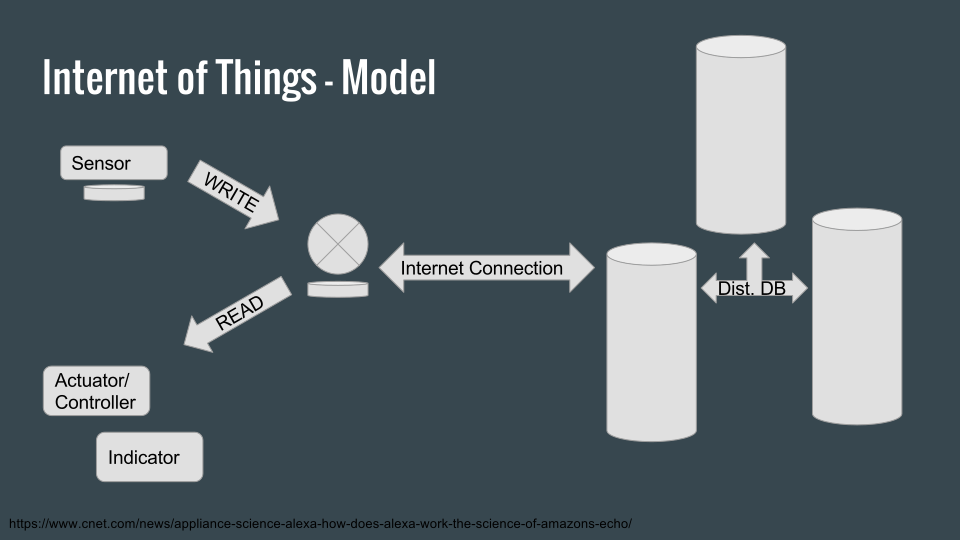
\includegraphics[width=7cm]{Figures/iot_original_model.pdf}
\caption{\gls{iot} Application...Although this isn't a rule, this represents a nominal "\gls{iot}" application.  Some measurement of interest, such as temperature is sensed, that raw data is stored and sent afar, and if desired, the user may also query for some kind of feedback or indication.}
\label{fig:iot_original_model}
\end{figure}

\begin{figure}[h]
\centering
\includegraphics[width=7cm]{Figures/iot_modified.pdf}
\caption{\gls{iot} Application with Thicker Clients...Depending on the application, using a distributed database on thicker clients in-situ may suitably replace a remote database operating in a remote location.  From an operational standpoint, the pipeline may be unreliable, resulting in a loss of data.  From a security standpoint, this pipeline may be subject to undesired third-party monitoring.}
\label{fig:iot_modified}
\end{figure}

\label{where a distributed database fits in}

At the time of this writing, Cassandra, or other distributed databases, is used as a back-end database operating on powerful, but stationary nodes.  This paper explores the idea of moving toward a more in-situ database, where the sensing nodes may also contain serve as mechanisms for storage and do not require a pipeline to another datacenter, a pipeline that from an operational perspective, represents a single point of failure, or from a security perspective, a threat to privacy.

The next few sections map this general concept to some particular applications that are a bit easier to digest.

\subsection{WiFi Collection, Mapping and Analysis}
\subsubsection{WiFi Sniffing, Collection}
WiFi (802.11) sniffing, or war-driving, has been explored by a number of enthusiasts, both in and out of the academic realm.  These techniques for WiFi sniffing, at least on the front-end, is well-documented and thus represents a low barrier to entry for initial operations, often just requiring a specific WiFi chipset, such as the ALFA card, and open-source software.  One example that has been well-documented goes by the clever name of "Snoopy" \cite{SensePostFramework}.  Snoopy  provides a framework for collecting WiFi data and observing with another handy piece of software, Maltego.  Of course, a multitude of other software exists.  For example, one can sniff wireless traffic by using software Aircrack-ng \cite{Aircrack-ng} or Airsnort \cite{AirSnortHomepage}.  All this goes to show that it really doesn't take much to set up a sensor to get all the valuable information radiating throughout.  However, although sensing the data is easy, the subject of storage has not been fully explored with respect to the selling points mentioned above.  Investigating the limits of storage operations is key to unlocking realistic aspirations and application development.

\subsubsection{WiFi Mapping}
It may worth noting one off-shoot of the WiFi sniffing mentioned above: WiFi mapping.  There is much interest in WiFi mapping: Who doesn't want extra assurance of where they are in the world (especially if the GPS goes out)?  There has been much work done with respect to WiFi mapping.  Argos \cite{Rose2010MappingArgos} describes a similar system of a distributed system, but there is no mention of Cassandra or any distributed database, which may serve as an improvement on such a sensor network.  Wigle.net \cite{WiGLE:Mapping} is an aggregate map that distributes a smart-phone application to collect GPS coordinate-Access Point pairs, but relies on a central database, and has an unreliable user base and irregular sampling and update frequencies (Relying on the public will often do that, unfortunately.).  Heat Mapper \cite{HeatMapperOffices} is partially free and commercial software that can generate a heat map for a small room or office.  Wi2Me \cite{Castignani2012Wi2Me:Networks} performs this mapping as well, with an emphasis on performance and data throughput.  It uses an instance of SQLite to store the traces on the individual's smart-phone, but again, none of these make use of a distributed database like Cassandra as part of the sensor network.  Once again, this is a realm that may benefit integration with distributed databases, expanding the range possible node types, or both.  However, there are limits that have to be anticipated.  This paper aims to add a piece to that expectation management.

\subsection{WiFi/Wireless Crowd Detection}
There is also considerable interest in crowd detection and related data gathering.  Privacy implications notwithstanding, this kind of data can give a marketing-type a sense if certain areas are popular or versus other areas, or if certain paths are well-traveled or not.  The way WiFi broadcasts \gls{ssid}s in plain text, crowds can even be characterized as to whether individuals connect to similar access points or not.  The data can indicate whether you have a crowd of people from a certain country, a crowd of people who know each other or maybe just a crowd of strangers.  It can add assurance to more primitive forms of tracking, such as person-by-person registration.  Informally, some have even reported to make art exploiting this mechanism \cite{KeebleCasual2013}, and not surprisingly, there are numerous claims that members of the public are routinely tracked via commercial entities via WiFi \cite{HaighTrackingConnected}. There have been more academic efforts to track crowds as well, notably a university campus and a music festival in \cite{Bonne2013WiFiPi:Events} and an airport in \cite{Schauer2014EstimatingBluetooth}.  In \cite{Bonne2013WiFiPi:Events}, data travels through \gls{gsm} to a central node, but does not use any kind of distributed database, like Cassandra.  There are commercial entities that claim to track crowds and report data, namely "Bluemark" \cite{SchiphorstBlueInnovations}.  Here as well, a central server is utilized to collect the data.
Users then reportedly log into the web to view the metrics.  According to their marketing literature, they do use Raspberry Pi, but not for data storage. Paper \cite{ChilipireaPresumablyWiFi} used this product line for their tests. Although WiFi utilizes \gls{mac} addresses supposedly unique to each device, research has found that this leaves more to be desired for many applications, namely crowd-tracking.  For instance, some devices have been reported to change their MAC addresses \cite{ChilipireaPresumablyWiFi}.  There exist a number of papers that explore characterizing mobile devices and their users at the individual level \cite{Pang2007802.Fingerprinting, Chernyshev2016ServiceChallenges, Cunche2014LinkingRequests, Du2016EV-Linker:Matching, Cunche2012IRequests, Luzio2016MindRequests, Musa2012TrackingMonitors} and propose techniques to better prepare data for analysis \cite{ChilipireaPresumablyWiFi}.  What is clear in the subtext of all these papers, is that these types of application research can only benefit from a wider choice in nodes, and a wider choice storage options as well as a reasonable amount of foresight into their performance.  In all of these, however, distributing the stored data among the nodes, like with Cassandra is either not used or not mentioned.  Many utilize a central server that represents a single point of vulnerability.

\subsection{CBIR and others and summary statement on application space}
The motivation for WiFi mapping can also be extended to other types of mapping, such as \gls{cbir}.  Paving the way for feasible, desirable in-situ data storage increases the portability and development of these and many more applications.

The experiments that follow read and write random data in the context of a meaningless, and rather ho-hum schema, but the experiments were done with the following in mind: A schema supporting any of these up-and-coming applications could be substituted in instead, and ideally with predictable results.

\section{Representative Technologies}

\subsection{Cassandra}
\label{Cassandra}
%NEED FOR DISTRIBUTED DATABASE
A distributed database offers a trade space among consistency, availability, and partition tolerance.  Mostly this means that a system of nodes can still operate as expected even if there is a loss of one or two nodes.  There is no shortage of distributed databases to choose from, but Cassandra is widely used  and is known to have a high write throughput \cite{Cooper2010}.  Cassandra specifies the “latest” versions of both “Java 8” and “Python 2.7”.  In turn, Java can run on Windows, Mac OS X, Linux, and Solaris \cite{CassandraHardwareWiki}.

%SELECT THE REPRESENTATIVE – CASSANDRA AND WHY?
Cassandra is a widely used distributed \gls{nosql} database with many use cases \cite{Lakshman2010CassandraSystem} and boasts a high write throughput. Not only has Cassandra been reportedly been used in practice \cite{ApacheCases}, but has been, using the Yahoo Cloud Services Benchmark \cite{YahooBenchmark}, formally evaluated in scholarly literature against other databases such as MongoDB and proposed as the NoSQL database of choice in the Internet of Things and distributed sensor networks \cite{Abramova2013NoSQLCassandra}.

%SET OF HARDWARE/OS THAT SUPPORT CASSANDRA
If possible, it is important to get realistic expectation from available specifications whether or not the database of interest, Cassandra, would be supported by the node of interest, in this case Raspberry Pi. At the time of this writing, Cassandra specifies it is supported by the “latest” versions of both “Java 8” and “Python 2.7” \cite{CassandraHardwareWiki}.  In turn, Java can run on Windows, Mac OS X, Linux, and Solaris.  Raspbian, a Linux-based operating system, can be run on Raspberry Pi.  In addition, there have been credible claims of Cassandra being used on Raspberry Pi \cite{VanRyswykMulti-DatacenterPis,SercelCassandraMedium}, but to the author's knowledge, no white paper with the details exists.

This author's interest in Cassandra lies in the fact that Cassandra is a distributed database used in practice for cloud computing.
Although it describes itself as a \gls{nosql} database, the interface allows for \gls{sql} commands and has a Python \gls{api}.
Cassandra allows for configuration of distributed systems parameters, such as replication factor, but detailed knowledge of distributed systems protocols is not critical for operation.

%But in a way, this is the simplified version of the application that this is testing.
The aim of this paper is to examine Cassandra's performance coupled with a simplified Wi-Fi collection and analysis application, where the nature of link nodes may be less reliable than wired Ethernet.

From an experimental standpoint, the distributed nature of a Cassandra "keyspace" lies in four parameters \cite{CassandraDummies}: cluster size (the number of nodes), replication factor (configured in software), write level (configured in software), and read level (configured in software).
As alluded to in section \ref{Factors Held Constant}, these factors will be held constant for this experiment.

\subsection{Raspberry Pi 2}

The Raspberry Pi 2 (Model B) \cite{RaspberryB} is a low-cost computer designed sold from the United Kingdom.
It can be described as a motherboard for a about the size of a 3x5 index card and has been available since February 2015.
This experiment is interested in the Raspberry Pi 2 as a representative of the low-cost hardware domain, which implies low cost, low power consumption, and low in terms of size and weight.

This author's interest in the Raspberry Pi 2 is that its ARM Cortex-A7 processor and 1GB \gls{ram} \cite{RaspberryB} makes it a key representative of the low-cost hardware domain and the \cite{iot}.
The Raspberry Pi 2 has cost as low as 35 \gls{usd} \cite{RaspberryPi}.
It is lightweight and has limited power consumption \cite{RaspberryB}.
Constraints on size, weight, power, and cost can all be barriers to entry for applications seeking computing nodes.

Expanding this experiment, to say the BeagleBone black \cite{BeagleBoard.orgBlack}, is in touch with the spirit of this experiment but outside the scope of this paper.  A number of possible alternatives is listed in Table \ref{table:low_cost_hardware}

\begin{table}
\begin{tabular}{|| p{2cm} | p{4cm} | p{2cm} | p{3cm} | p{1.5cm} ||}
\toprule
 Name	& CPU	& RAM &	DISK &	Price \\
\midrule
Banana Pi M3 &	Octa-core 1.8GHz CPU &	2 GB RAM &	8 GB eMMC flash storage	& 73.00 \\
\hline
CHIP &	R8 1GHz &	512 MB &	4 GB	& 9.00 \\
\hline
VoCore &	360 MHz MIPS CPU &	32 MB &	8 MB Flash	& 20.00 \\
\hline
Arduino INDUSTRIAL 101 &	Atheros AR9331 Processor &	64 MB &	16 MB Flash	& 40.00 \\
\hline
NanoPi 2 Fire &	Samsung S5P4418 quad-core ARM Cortex-A9, 1.4 GHz & unk &	1 GB MicroSD card & 22.99 \\
\hline
NanoPC-T3 &	Samsung S5P6818 octa-core ARM Cortex-A53 up to 1.4 GHz & 1-2GB of RAM & 8GB of flash storage & 60.00 \\
\hline
Intel Edison with Kit for Arduino & Dual-core, dual-threaded Intel Atom CPU with a 32-bit Intel Quark microcontroller & 1GB of RAM & 4GB of flash storage & 92.00 \\
\hline
cloudBit & Freescale i.MX23 ARM926EJ-S processor & 64MB of RAM & 4GB SD Card & 59.95 \\
\hline
Parallella & 16-core Epiphany RISC SOC & unk & unk & unk \\
\hline
Zynq SOC & (FPGA + ARM A9) & 1GB SDRAM & Micro-SD storage & 99 \\
\hline
PixiePro & Freescale i.MX6Q Soc Quad Core ARM Cortex-A9 up to 1GHz & 2GB of RAM& SD Card	& 129.95 \\
\hline
Raspberry Pi & 900 MHz quad-core ARM Cortex-A7 CPU & 1GB RAM & MicroSD Card & 35.90 \\
\bottomrule
\end{tabular}
\caption{Raspberry Pi Alternatives, Depending on Application}
\label{table:low_cost_hardware}
\end{table}

%\subsection{Wireshark software and PCAP files}

%A PCAP file stores networking packets and is a "main capture file format" \cite{tcpdumpTcpdump/LibpcapRepository}.
%In this case, the PCAP file is used as a tool in the benchmark, a means to an end.

%Commonly associated with PCAP files, and used by this author is the Wireshark software \cite{WiresharkDeep.}.
%This was used to view and confirm that the PCAP files were generated to taste.

%Not even a vague familiarity of these is needed to understand the experiment, but they are a fundamental part of the custom benchmark of choice. 